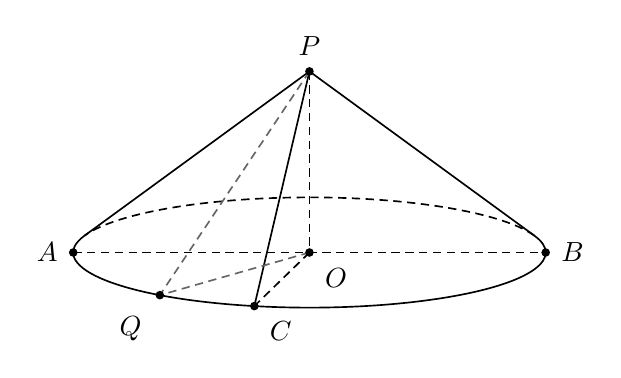
\begin{tikzpicture}[x=1cm,y=1cm,line width=.6pt]
\tikzset{pt/.style={circle,fill=black,inner sep=1.1pt}}
% cone and source auxiliary points on the visible base arc
\coordinate (P) at (0.0000000000,2.3000000000);
\coordinate (O) at (0,0);
\coordinate (A) at (-3,0);
\coordinate (B) at (3,0);
\coordinate (C) at (-0.7000000000,-0.6806777668);
\coordinate (Q) at (-1.9000000000,-0.5417153824);
% base ellipse: front solid (180->360), back dashed
\draw[black] (-2.857682908723,0.213043478261) arc[x radius=3,y radius=.7,start angle=162.281068126593,end angle=377.718931873407];
\draw[black,densely dashed] (2.857682908723,0.213043478261) arc[x radius=3,y radius=.7,start angle=17.718931873407,end angle=162.281068126593];
% diameter + axis + radius
\draw[black,densely dashed] (A)--(B);
\draw[black,densely dashed] (P)--(O);
\draw[black,densely dashed] (O)--(C);
% generators
\draw[black] (P)--(-2.857682908723,0.213043478261);
\draw[black] (P)--(2.857682908723,0.213043478261);
\draw[black] (P)--(C);
% source auxiliary radii OQ and PQ

\draw[black!60,densely dashed] (O)--(Q);
\draw[black!60,densely dashed] (P)--(Q);
\foreach \p in {P,O,A,B,C,Q}{\node[pt] at (\p) {};}
\node[above=2pt] at (P) {$P$};
\node[below right=2pt] at (O) {$O$};
\node[left=2pt] at (A) {$A$};
\node[right=2pt] at (B) {$B$};
\node[below right=2pt] at (C) {$C$};
\node[below left=2pt,xshift=-1.0pt,yshift=-2pt] at (Q) {$Q$};
\end{tikzpicture}

